\documentclass[conference]{IEEEtran}
\IEEEoverridecommandlockouts
% The preceding line is only needed to identify funding in the first footnote. If that is unneeded, please comment it out.
\usepackage{cite}
\usepackage{amsmath,amssymb,amsfonts}
\usepackage{graphicx}
\usepackage{textcomp}
\usepackage{xcolor}
\usepackage{amsmath}
\usepackage{algorithm}
\usepackage{algorithmicx}
\usepackage{algpseudocode}
\usepackage{multirow}

\makeatletter
\def\BState{\State\hskip-\ALG@thistlm}
\makeatother

\def\BibTeX{{\rm B\kern-.05em{\sc i\kern-.025em b}\kern-.08em
    T\kern-.1667em\lower.7ex\hbox{E}\kern-.125emX}}
\begin{document}

\title{Retrieval Augmented Generation}

\author{\IEEEauthorblockN{Duarte Santos}
    \IEEEauthorblockA{\textit{DETI} \\
        \textit{Universidade de AVeiro}\\
        124376 - duartevsantos@ua.pt}}
% Monograph about RAG (Retrieval Augmented Generation)

\maketitle

\begin{abstract}
    Retrieval Augmented Generation (RAG) is a model that combines the strengths of retrieval-based and generation-based models (GPT \cite{noauthor_chatgpt_nodate}, Llama \cite{noauthor_llama_nodate}).
    It uses a retriever to find relevant information from a large corpus and a generator to produce the final output.
    This model has been shown to outperform previous models in several tasks, such as question answering and text summarization.
    In this monograph, I present an overview of the RAG model, its architecture, and its training process.
    It's also discussed the advantages and limitations of the model and present some of the most recent research in the field.
    Finally, I present some ideas for future research and discuss the potential impact of RAG on the field of natural language processing.
\end{abstract}

\begin{IEEEkeywords}
    Retrieval Augmented Generation, RAG, Natural Language Processing, Question Answering, Text Summarization
\end{IEEEkeywords}

\section{Introduction}
In 2020 Patrick Lewis \cite{lewis_retrieval-augmented_2021}, proposed a novel framework called RAG
that combines information retrieval with generative models. The base idea was to retrieve relevant text passages
from large documents and use them to guide the LLMs generation process, leading to improved performance
in tasks like question answering about specific data. This approach leverages both explicit knowledge from retrieved
documents and the implicit knowledge encoded in language models, resulting in more accurate and
context-sensitive responses.

This came as a response to the limitations of LLMs. While LLMs have shown impressive results in
responding to general prompts at light speed, they still struggle with tasks
that require a deeper understanding of the context or specific knowledge that is not present in the training data.

\section{Why use RAG to enhance LLMs?}
LLMs can be outdated or biased in their responses, as they are trained on a fixed dataset and do not have access to new real-time information.
For example, if we ask \textbf{GPT-4o mini} who were the candidates in the 2024 USA presidential election and who won,
it will not be able to provide an accurate answer, as it was trained on data up to September 2021 (Figure \ref{fig:gpt4o_mini_response}).
RAG overcomes this problem using dynamic retrieval from current data sources.

\begin{figure}[htbp!]
    \centerline{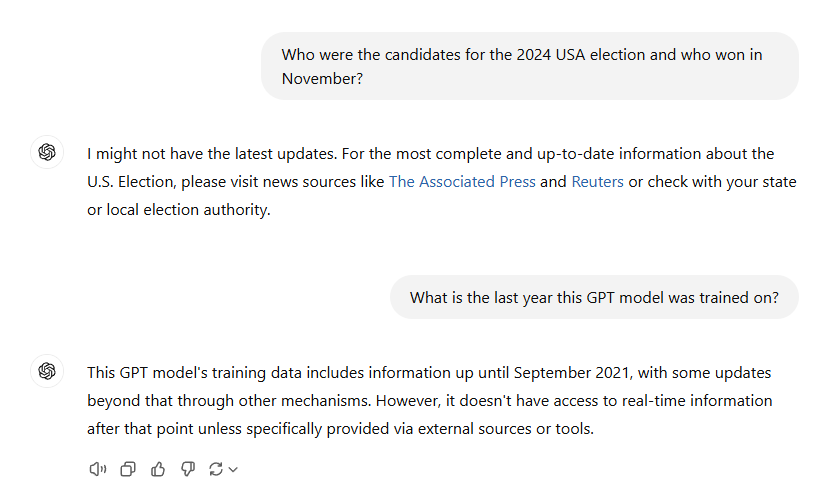
\includegraphics[width=0.5\textwidth]{images/gpt4o_mini_response.png}}
    \caption{GPT-4o mini response to the question "Who were the candidates for the 2024 USA election and who won in November?"}
    \label{fig:gpt4o_mini_response}
\end{figure}

Other limitation of LLMs is that when they don't have the necessary information to answer a question, they tend to generate text
that is not factually accurate or relevant to the query. This is known as \textit{hallucination} and can lead to misleading or incorrect responses.
RAG addresses this issue by adding quality context to the query.

\section{RAG Structure}
The basic structure of RAG involves three key components: indexing, retrieval and generation (Figure \ref{fig:rag_structure}).

For this structure to work, it is important to first collect and select a large
corpus of documents that will be used for retrieval. This corpus can be a collection of
Wikipedia articles, scientific papers, books, or any other type of text data that is relevant to the task at hand.
The quality of this corpus is crucial for the accuracy, as it will influence the responses generated by the model.

\begin{figure}[htbp!]
    \centerline{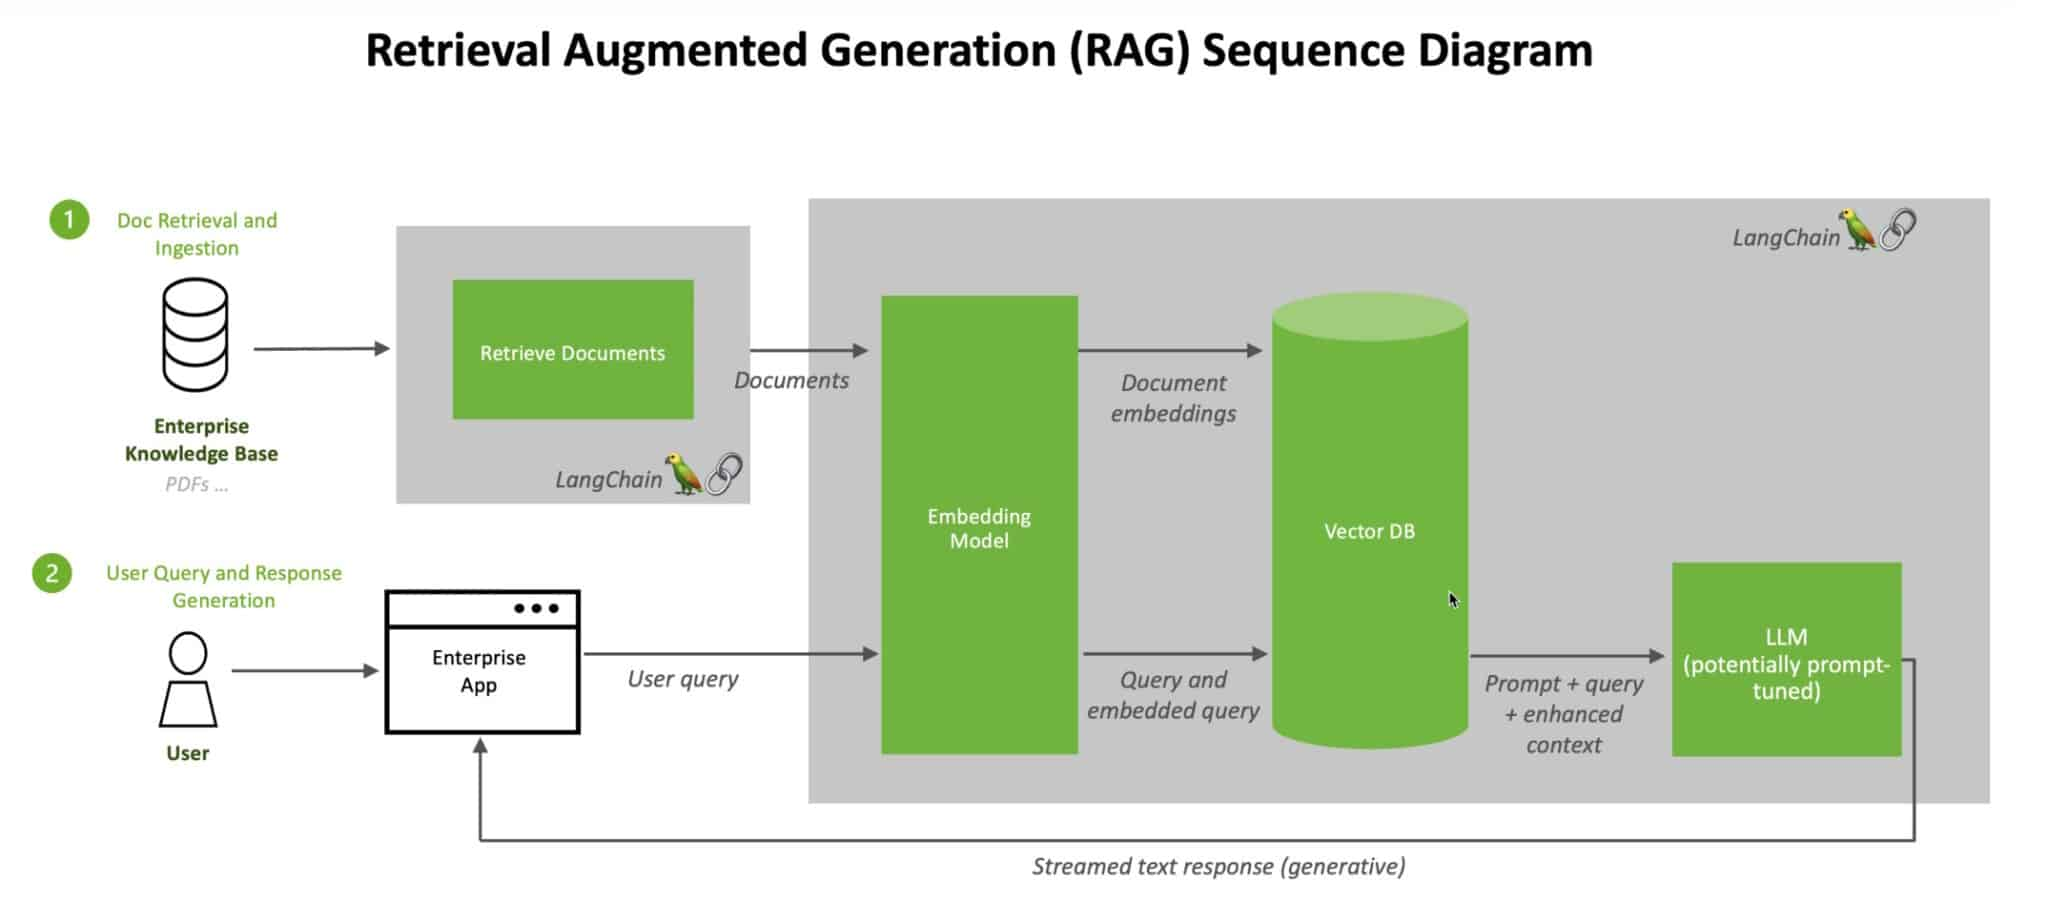
\includegraphics[width=0.5\textwidth]{images/NVIDIA-RAG-diagram-scaled.jpg}}
    \caption{RAG Structure by NVIDIA \cite{merritt_what_2024}}
    \label{fig:rag_structure}
\end{figure}

\subsection{Indexing}
Indexing is the process of converting each document from the corpus into an embedding,
typically using a transformer-based encoder or other embedding model.

This typically involves breaking down the documents into smaller, manageable
pieces called chunks. Each chunk is a segment of the document that can be independently processed and searched.
This helps in handling large documents by focusing on relevant sections rather than the entire document (Figure \ref{fig:indexing_diagram}).

This brings several advantages:
\begin{itemize}
    \item \textbf{Efficiency:} Searching for relevant chunks is faster than searching for entire documents.
    \item \textbf{Scalability:} Indexing and searching chunks is more scalable than indexing and searching entire documents.
    \item \textbf{Flexibility:} Chunks can be processed in parallel, enabling more efficient use of computational resources.
    \item \textbf{Accuracy:} Chunks can be matched to the query more accurately, leading to better retrieval results.
\end{itemize}

These embeddings are then stored in a vector database, enabling quick similarity
searches to retrieve the most relevant document chunks based on their semantic content.

\begin{figure}[htbp!]
    \centerline{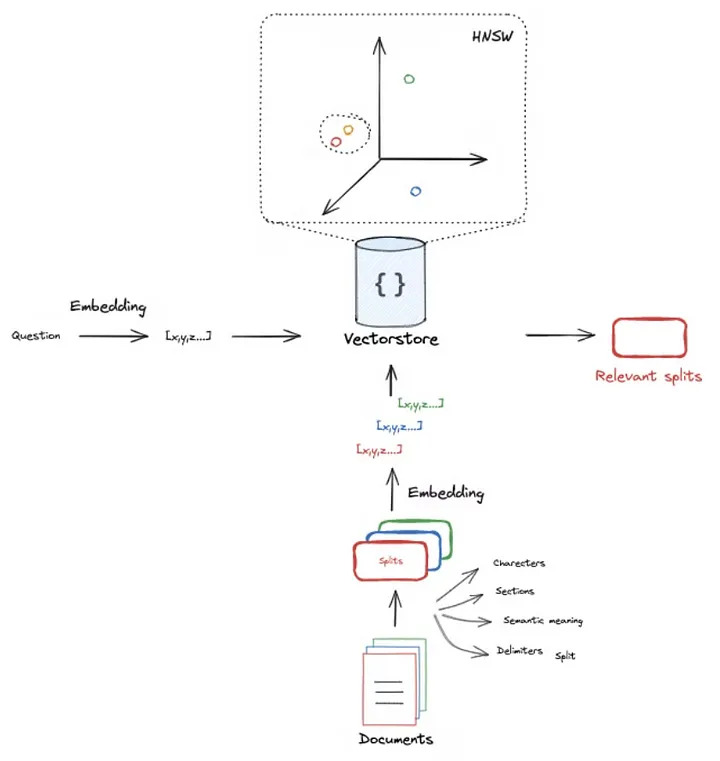
\includegraphics[width=0.5\textwidth]{images/indexing_diagram.jpg}}
    \caption{Indexing process diagram \cite{bavli_rag_2024}}
    \label{fig:indexing_diagram}
\end{figure}

\subsection{Retrieval}
The retrieval component is responsible for finding the most relevant embeddings (chunks) from the vector database
based on a given query. To do so, the query is converted into its vectorized form using
the same embedding model used for indexing and then is calculated the similarity between the query and each chunk in the database.

The most common similarity metric used is the cosine similarity, which measures the cosine of the angle between two vectors.
The higher the cosine similarity, the more similar the two vectors are.
The top-k most similar chunks are then retrieved and passed to the generation process.

\subsection{Generation}
The generation process happens after the retrieval has returned the most relevant chunks.
Then these chunks and the query are put together in a prompt template that is fed into the LLM (GPT, Llama etc...).
The LLM then do its job and generates the final output, which is the answer to the query with all the
contextual information retrieved from the corpus.

\section{RAG pros and cons}

\subsection{Advantages}
\begin{itemize}
    \item \textbf{Enhanced Accuracy:} By leveraging specific, up-to-date documents, the model has more reliable context.
    \item \textbf{Reduced Hallucination:} Retrieval-based information provides
          factual grounding and minimizes fabricated outputs.
    \item \textbf{Scalability:} Splitting documents into chunks and indexing them allows fast and efficient searches across large corpora.
    \item \textbf{Modularity:} The retrieval and generation components can be updated or replaced independently, making the overall system adaptable.
\end{itemize}

\subsection{Limitations}
\begin{itemize}
    \item \textbf{Complex Architecture:} Designing and maintaining both the retriever and the generator can be more involved than using a single large model.
    \item \textbf{Embedding Quality Dependence:} The system relies on highly effective embeddings; suboptimal encodings may negatively impact retrieval performance.
    \item \textbf{Potential for Irrelevant Context:} If the retrieval step fetches imprecise chunks, the generation could incorporate misleading information.
    \item \textbf{Training Data Bias:} The model may inherit biases from the training data, which could be exacerbated by the retrieval process.
\end{itemize}

\section{RAG use cases}
RAG has shown promising results in several natural language processing tasks, in different
domains and applications. Some of the most notable use cases include:
\begin{itemize}
    \item \textbf{Customer Support Chatbots:} Dynamically accesses knowledge bases to respond with up-to-date and relevant information, reducing hallucination.
    \item \textbf{Academic Research Assistants:} Retrieves scientific papers or articles when generating summaries or literature reviews, ensuring higher factual grounding.
    \item \textbf{Enterprise Document Search:} Locates policies, contracts, or guidelines and incorporates them into query responses, improving internal knowledge retrieval.
    \item \textbf{Healthcare Q\&A Systems:} Retrieves validated medical texts to answer patient inquiries with reliable references, minimizing misdiagnoses from misinformation.
\end{itemize}
Those are just a small fraction of the possible applications of RAG, as the model can be adapted to any domain and be
incorporated into a wide range of systems that require accurate and context-aware responses.

\section{Future of RAG}
As RAG continues to evolve, several key areas of exploration are likely to drive future developments. One such area involves refining retrieval strategies through more advanced indexing mechanisms and hybrid methods that combine symbolic and dense embeddings. This has the potential to improve the precision and recall of relevant documents, particularly for specialized domains where standard embeddings may not capture nuanced terminology.

Another direction is adaptive index updates, enabling dynamic incorporation of new data without requiring a full reindexing process. This would allow real-time retrieval from continually changing knowledge bases such as news feeds, social media platforms, or specialized databases in fields like genomics and finance. By integrating incremental training methodologies, RAG systems could rapidly adjust to domain shifts and emerging events, curtailing outdated responses.

Cross-lingual retrieval is also a promising avenue, where a single system could handle queries in multiple languages, retrieving and synthesizing evidence from diverse multilingual sources. Combining this with multimodal data—such as images, audio, or structured metadata—could further enhance context-aware responses. For instance, a healthcare chatbot could retrieve medical images and relevant text to better support diagnostic tasks.

Finally, efforts to align RAG with human values and ethical considerations will be essential. Building mechanisms for controlling or filtering retrieved content, ensuring user privacy, and mitigating issues of bias remain open research challenges. Addressing these concerns will help foster greater trust and reliability in RAG-driven applications, paving the way for broader adoption in critical domains like finance, healthcare, and policy-making.

\section{Conclusion}
RAG offers a flexible and robust approach to improving LLM responses by leveraging retrieval-based context.
Its modular design and grounding in updated data help mitigate hallucination and enhance factual accuracy.
While it introduces complexities in architecture and embedding quality, it shows strong potential across multiple domains.
Future work on better retrieval techniques and handling evolving data will further strengthen the reliability and applicability of RAG.


\bibliographystyle{IEEEtran}
\bibliography{references}

\end{document}
